\chapter{Processor Core}

Chapter \ref{chp:system-overview} describes how vector graphics are supported and integrated into the \vthreek architecture.
This chapter elaborates on how the processor core is designed, focusing especially on features directly related to vector graphics.

\section{The \vthreek processor}

The processor core is the main processing and control unit in the \vthreek architecture.
As depicted in figure \label{fig:system-overview}, the processor core reads instructions from the instruction memory, and writes/reads data to/from the data and scene memories.
The processor core is designed as a multi-cycle, MIPS-inspired processor with extra features added to support processing of vector graphics.
When planning which features to include and which techniques to utilize, the group considered features like pipelining and even multicore designs to improve performance.
In the end, the decision was made to make the initial design simple, but keep efficiency and performance in mind.

\begin{figure}[H]
    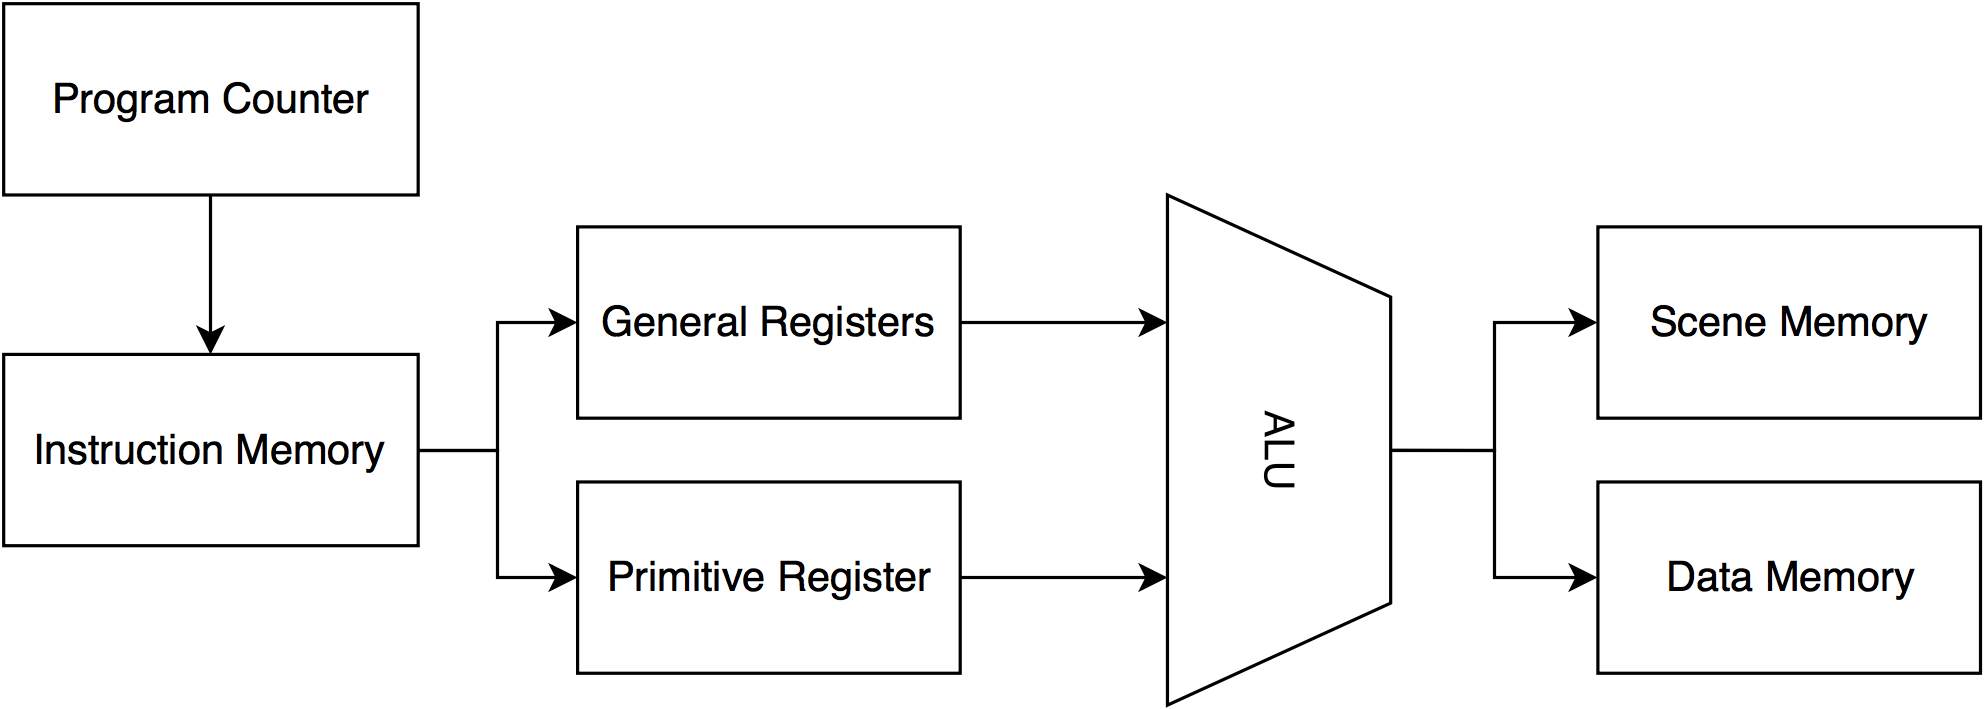
\includegraphics[width=\linewidth]{images/core-components.png}
    \caption{Overview of the main components in the processor core.}
    \label{fig:core-components}
\end{figure}

Figure \ref{fig:core-components} shows how data flows through the subcomponents of the processor core.
In addition to the components in the figure, the core includes a control unit.
Each component is described in detail in their respective section below, the following is a short introduction to their responsibilities.

\begin{description}
    \item[Program counter] \hfill \\
        The program counter keeps track of the address of the next instruction to be executed.
        Depending on the instruction currently being executed, the program counter is either incremented or overwritten.
    \item[Control] \hfill \\
        The control unit keeps track of the state of the processor, namely fetch, execute and stall, and issues the appropriate control signals to the other components.
    \item[Register] \hfill \\
        The register bank is the short term memory of the core, feeding operands to the ALU, and recieving data which may be stored based on the control signals.
    \item[ALU] \hfill \\
        The ALU performs operations on the data it receives from the register unit and outputs the result.
    \item[Primitive Register] \hfill \\
        The primitive register is a special purpose register, containing the vector primitive that the core is currently processing.
\end{description}

\section{Instruction Format}

Instructions in the \vthreek architecture are 32 bits wide.
As opposed to the MIPS architecture, they can't all be grouped into categories based on their format.
They do however share some common traits.
All instructions start with an 6-bit opcode, a unique identifier for each instruction.
The remaining bits are used either to address registers, to encode immediate values or as a combination.
Some instructions also have don't care bits, parts of the instruction that can be either 1 or 0 without influencing the outcome of execution.
For instructions that address one or more registers, a general convention of using the five bits directly after the opcode for the destination register and addressing source registers in successive five bit chunks.
Figure \ref{fig:instruction-format} shows how various parts of an instruction word is utilized.

\begin{figure}[h!]
    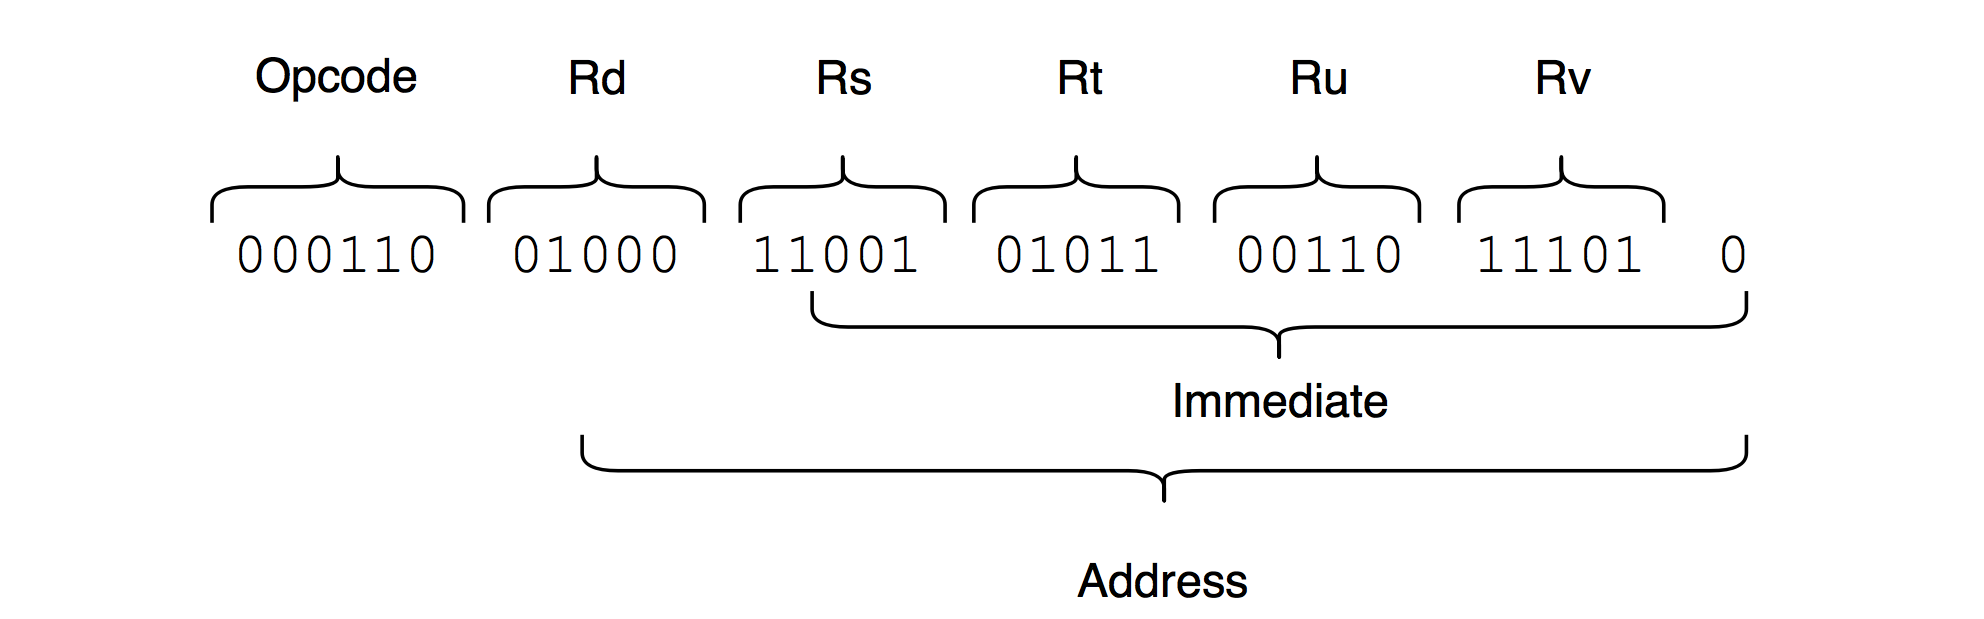
\includegraphics[width=\linewidth]{images/instruction-format.png}
    \caption{\vthreek instruction format.}
    \label{fig:instruction-format}
\end{figure}

As an example, the \texttt{jmp} instruction is encoded with the opcode \texttt{000001}, seven don't care bits followed by the 19-bit jump target.
The \texttt{bezcube} instruction initializes a cubic Bézier primitive into the primitive register, reading the coordinates of the four control points from four general purpose registers.
With 32 general purpose registers, five bits are needed to address them.
That means that the \texttt{bezcube} instruction is encoded with its six bit opcode, \texttt{000111}, followed by five don't care bits, then four 5-bit chunks, one for each register.
The final bit is also don't care.

\section{Data Path}

\begin{figure}[h!]
    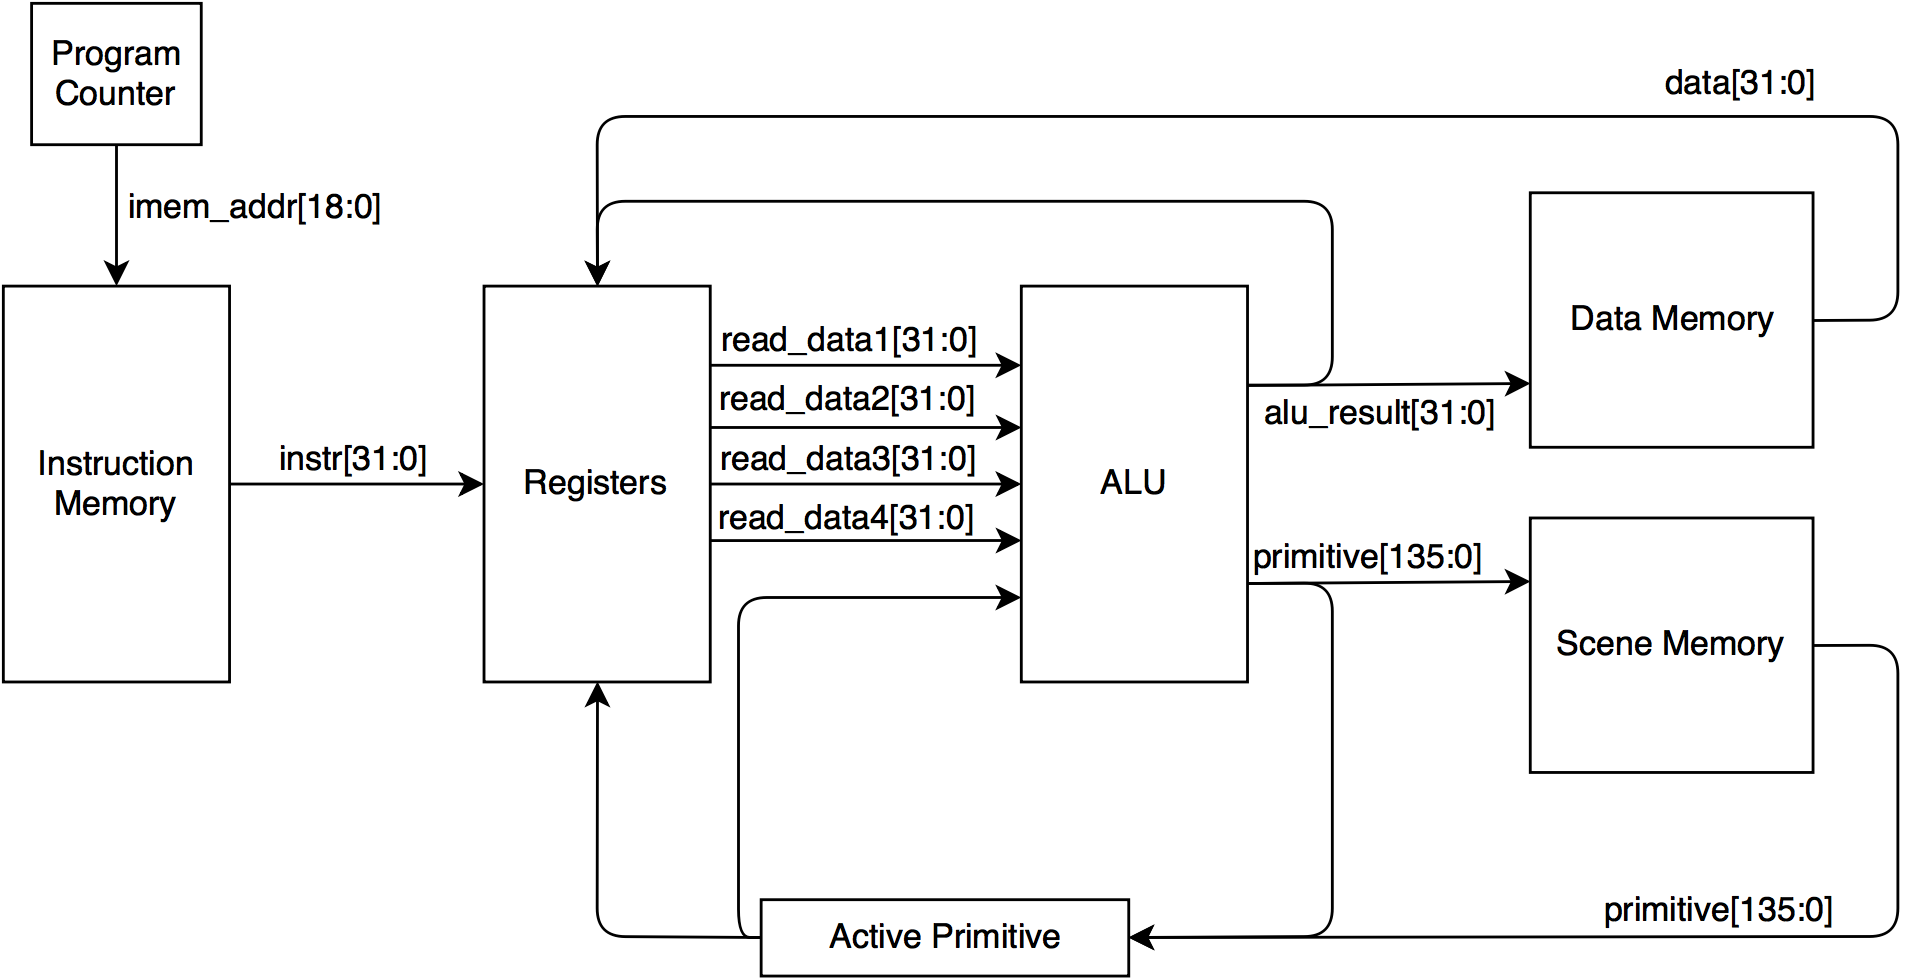
\includegraphics[width=\linewidth]{images/Data_path.png}
    \caption{RTL sketch of the data path.}
    \label{fig:datapath}
\end{figure}

The data path 

\section{Control Path}

\begin{figure}[h!]
    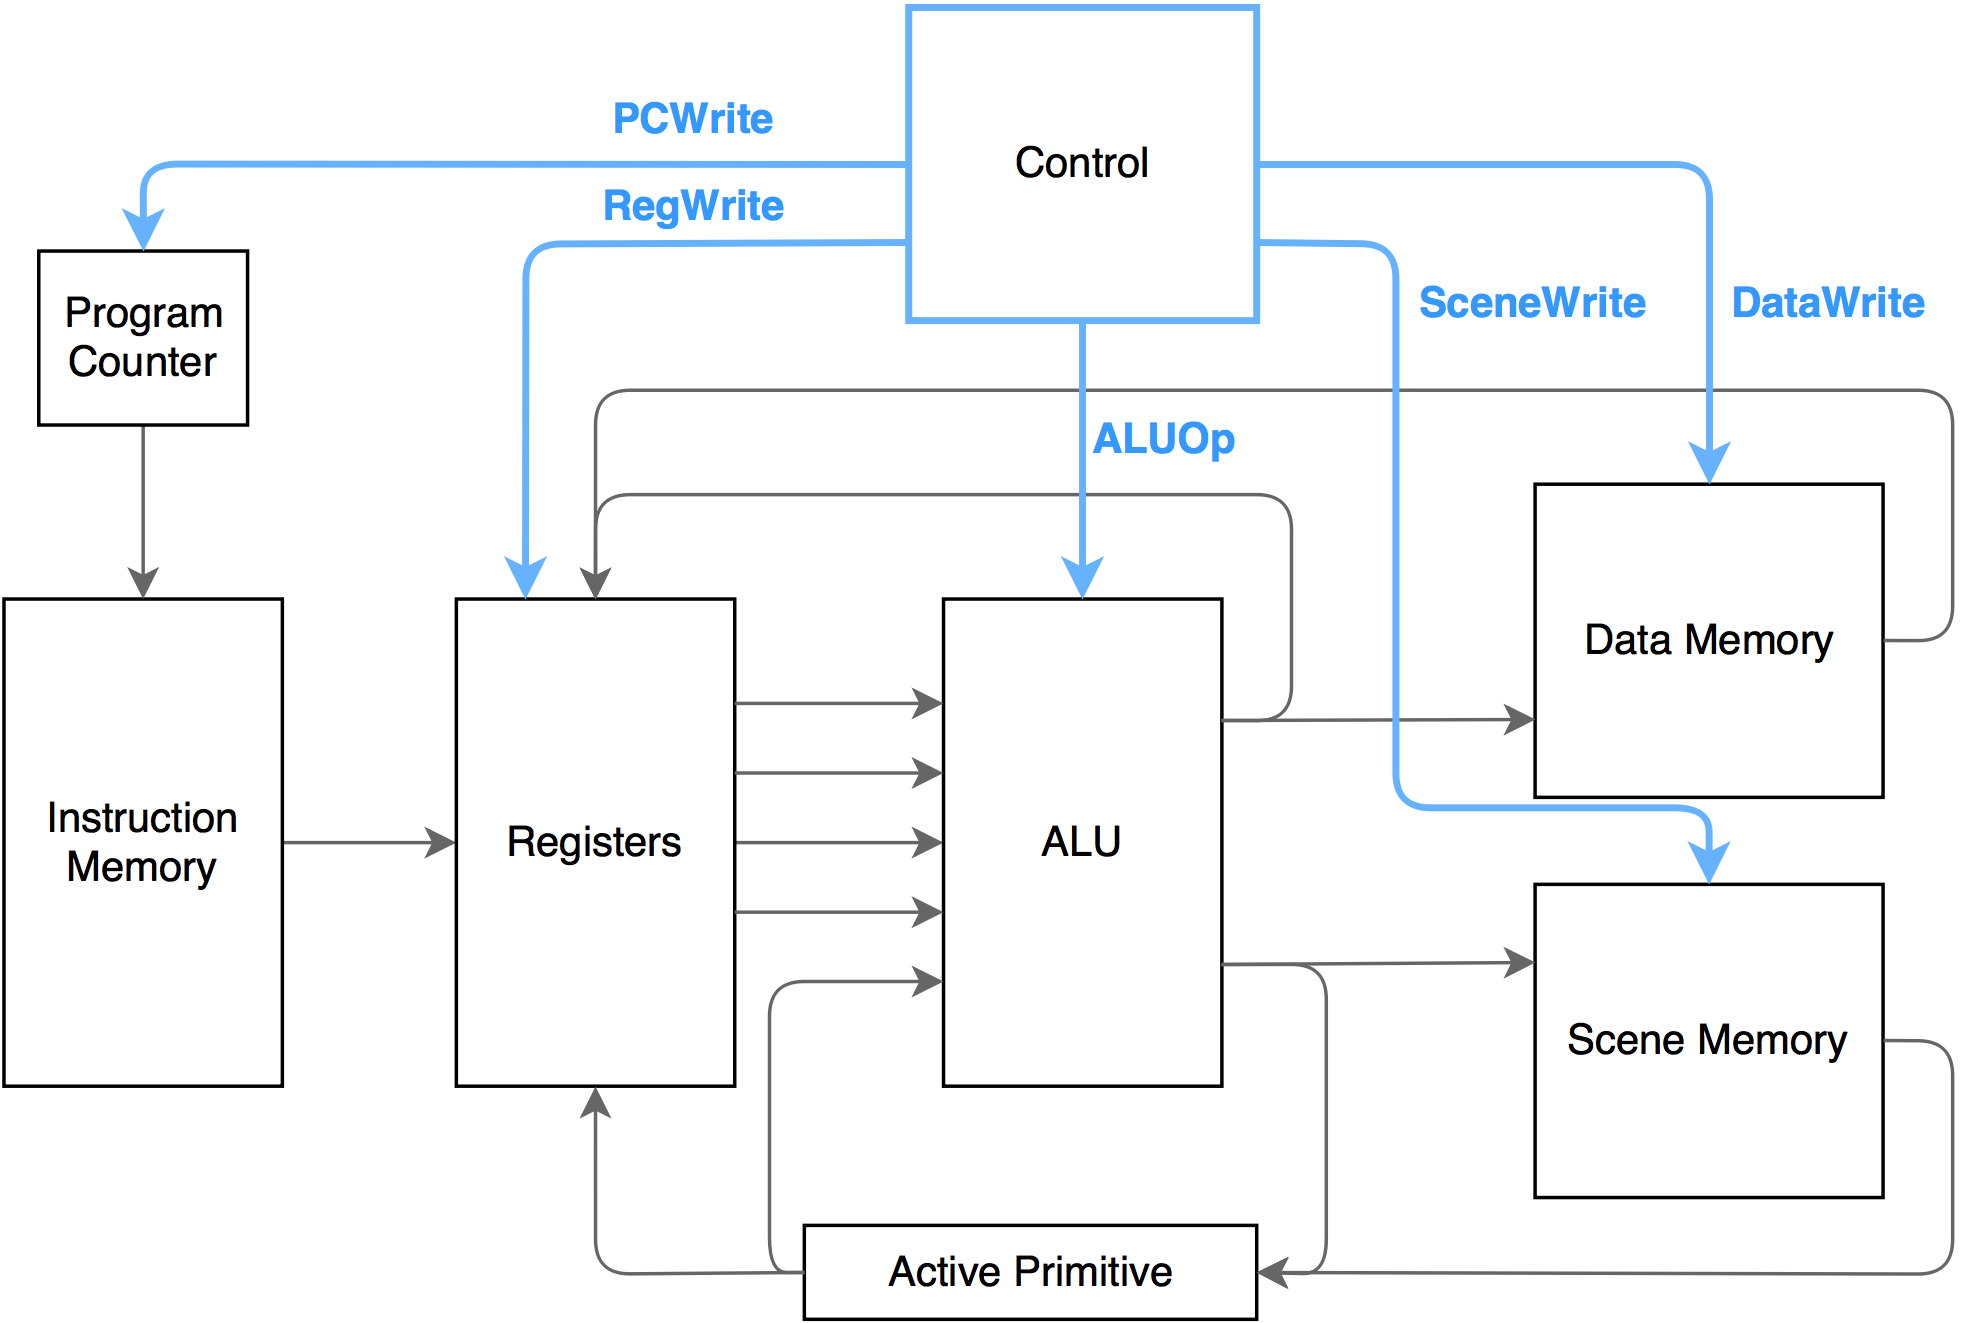
\includegraphics[width=\linewidth]{images/Control_signals.png}
    \caption{RTL sketch of the control path.}
    \label{fig:controlpath}
\end{figure}

